    \begin{figure}[H]
    \centering
    \caption{Exemplo de figura}%
    \label{fig:Metodologia.PNG}
    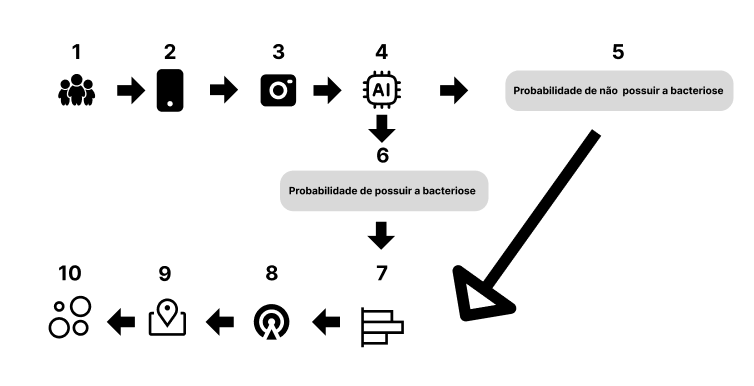
\includegraphics[scale=0.9]{Metodologia.PNG}
    \SourceOrNote{Autoria Própria (2024)}
    \end{figure}

Imagem 1 e 2:
Inicialmente, o usuário acessa o aplicativo e realiza seu cadastro fornecendo informações pessoais básicas. Esse cadastro é necessário para permitir o uso das funcionalidades do sistema e o armazenamento de dados associados.

Imagem 3:
Após o login do usuário, o mesmo interage com uma interface que permite o acesso à câmera do dispositivo. Essa etapa é fundamental para a captura da imagem da folha de mandioca, que futuramente será analisada a presença da bacteriose na folha.

Imagem 4:
O usuário realiza a captura de uma imagem da folha de mandioca, que deve seguir orientações específicas fornecidas pelo aplicativo, como foco e iluminação adequados, para garantir a maior precisão na análise.

Imagem 5:
Após a captura da imagem, o sistema de inteligência artificial processa a imagem e calcula a probabilidade de presença da bacteriose Xanthomonas paesoli. Isso supondo que o algoritmo utilizado foi treinado com um banco de dados de imagens previamente classificadas, possibilitando uma análise precisa.

Imagem 6:
Caso a probabilidade de presença da bacteriose seja baixa, o sistema informa ao usuário que a planta está saudável, indicando a confiança dessa análise com base nos resultados do modelo.
Imagem 7:
Se a probabilidade de presença da bacteriose for elevada, o aplicativo informa o usuário sobre a possível presença da infecção.

Imagem 8:
Em caso de detecção da bacteriose, o sistema realiza o envio dos dados de geolocalização, capturados via GPS, para identificar o local exato onde a foto foi tirada.

Imagem 9:
O GPS do dispositivo registra com precisão a localização da planta examinada, armazenando as coordenadas geográficas no banco de dados para análises posteriores.

Imagem 10:
Os dados de geolocalização são processados para gerar um mapa de calor que representa as áreas com maior incidência da bacteriose. Este mapa visa ser atualizado em tempo real, com base nas imagens capturadas e processadas em diferentes localidades.
